\section{Continuous FEM on an Unstructured Grid}
To discretize in space we will be using the continuous finite element method with bilinear basis functions on an unstructured triangular mesh. The mesh is generated with the triangle library via a Delaunay triangulation algorithm. 
\par
To integrate over the triangles, we have implemented a 2nd degree Gaussian Quadrature approximation over the standard triangle,
\begin{align}
    \iint_{T_{st}} f(\xi, \eta) d\xi d\eta \approx \frac{1}{6}\left [ f\left( 0, \frac{1}{2} \right ) + f \left( \frac{1}{2}, 0 \right) + f \left( \frac{1}{2}, \frac{1}{2} \right)\right].
\end{align}
We are working with an unstructured grid of triangles, so we must additionally map nodes on the standard triangle to an arbitrary element. This is done by the \texttt{gaussNodes()} function in this \texttt{FEGrid} class. 
\begin{figure}[h]
    \centering
    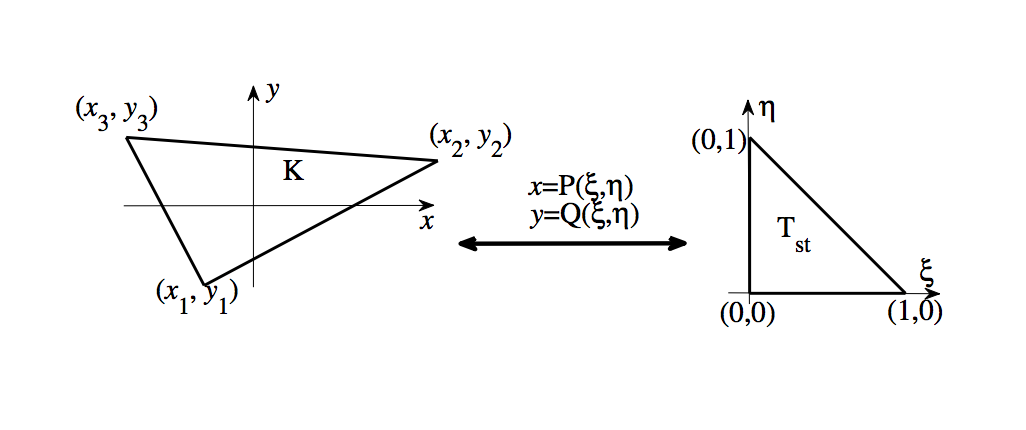
\includegraphics[width=0.75\textwidth]{fig/TriangleMapping}
    \caption{Linear mapping between an element K and the standard triangle}
    \label{fig:my_label}
\end{figure}
The mapping is given as follows
\begin{align}
    x &= P(\xi, \eta) = x_1 + \xi(x_2 - x_1) + \eta(x_3 - x_1) \\
    y &= Q(\xi, \eta) = y_1 + \xi(y_2 - y_1) + \eta(y_3 - y_1)
\end{align}
After applying the transformation we have,
\begin{align}
 \iint_{K} F(x, y) dx dy = \iint_{T_{st}}F(P(\xi, \eta), Q(\xi, \eta))|J(\xi, \eta)|d\xi d\eta
\end{align}
where $|J(\xi, \eta)|$ is the Jacobian of the transform which is equal to $2Area_K$. This gives the final quadrature rule as
\begin{align}
 \iint_{K} &F(x, y) dx dy = 2A_k\iint_{T_{st}}F(P(\xi, \eta), Q(\xi, \eta))d\xi d\eta \\
 &\approx \frac{1}{6}\left [ F\left( P(0), Q(\frac{1}{2}) \right) + F \left( P(\frac{1}{2}), Q(0) \right) + F \left( P(\frac{1}{2}), Q(\frac{1}{2}) \right)\right].
\end{align}

\section{Weak Form of NDA}
Similar to the higher order equation, we discretize  Eq. 4 via the continuous finite element method by multiplying by a test function and integrating over the domain. This gives the following weak form:

Find $\varphi_{d, g} \in W_D$ such that

  \begin{align}
  \left(D_\rg \nabla \varphi_\rg^{k+1/2}, \nabla \varphi^*_\rg\right)_\mathcal{D} &+ \left(\vec{\bf{D}_\rg}\varphi_\rg^{k+1/2} , \nabla \varphi^*_\rg\right)_\mathcal{D} +  \left(\sigma_{r,\rg} \varphi_{\rg}^{k+1/2}, \varphi^*_\rg\right)_\mathcal{D} = \nonumber \\
   \left(\sum\limits_{\substack{\rg'=1}}^\mm{g-1} \sigma_{\mm{s},\rg' \to\rg}\varphi_{\rg}^{k+1/2}, \varphi^*_\rg\right)_\mathcal{D} &+ \left(\sum\limits_{\substack{\rg'=\rg+1}}^\mm{G} \sigma_{\mm{s},\rg' \to\rg}\varphi_{\rg}^{k}, \varphi^*_\rg\right)_\mathcal{D} 
  + \left(S_\mathrm{f,g}, \varphi^*_\rg\right)_\mathcal{D}  \label{k1/2}
  \end{align}


The error (Eq. 8) is similarly discretized via CFEM.
  \begin{align}
  \left(\left< D\xi \right >\nabla \varphi_{\epsilon}^{k+1}, \nabla \varphi^* \right)_\mathcal{D} + \left(\left<\vec{\bf{D}\xi} \right>\varphi_{\epsilon}^{k+1}, \nabla \varphi^* \right)_\mathcal{D} &+ \left(\left<\sigma_r \right>\phi_{\epsilon}^{k+1}, \varphi^* \right)_\mathcal{D}  \nonumber \\= \left(\left<R^{k+1} \right>, \varphi^* \right)_\mathcal{D} &+ \left(\left<S_\mathrm{f,g} \right>, \varphi^* \right)_\mathcal{D} 
  \end{align}

\section{Weak Form of the Higher Order Equation}
We apply a finite element discretization to the higher order equation, SAAF, by first multiplying Eq. \ref{eq:SAAF} by a test function $\psi*$ and integrating over the domain $D$.

\begin{equation}
    \left ( -\vec{\Omega} \cdot \vec{\nabla}\frac{1}{\sigma_t}\vec{\Omega} \cdot \vec{\nabla} \psi, \psi* \right )_D + \left ( \sigma_t \psi, \psi* \right )_D = \left ( Q, \psi* \right)_D - \left ( \vec{\Omega} \cdot \vec{\nabla}\frac{Q}{\sigma_t}, \psi* \right)_D
\end{equation}
Integrating by parts,

\begin{align*}
        \left ( \vec{\Omega}\frac{1}{\sigma_t}\vec{\Omega}\cdot \vec{\nabla}\psi, \vec{\nabla}\psi* \right)_D &-     \left ( \vec{\Omega}\cdot \hat{n} \frac{1}{\sigma_t}\vec{\Omega} \cdot \vec{\nabla} \psi,\psi* \right)_{\Gamma} + \left ( \sigma_t \psi, \psi* \right )_D = \\
        \left ( Q, \psi* \right)_D &+ \left ( \vec{\Omega} \frac{Q}{\sigma_t}, \vec{\nabla}\psi* \right)_D - \left ( \vec{\Omega}\cdot \hat{n} \frac{Q}{\sigma_t}, \psi* \right)_{\Gamma} 
\end{align*}

This can be written in matrix form as
\begin{equation}
    (A - B + C)\psi = D - E
\end{equation}
where,
\begin{align*}
    A_{ij} &= \int_{D}\frac{1}{\sigma_t}\vec{\Omega}\cdot \vec{\Omega} \nabla \varphi_i \nabla \varphi_j dx \\
    B_{ij} &= \oint_{\Gamma} \frac{1}{\sigma_t}\vec{\Omega}\cdot \vec{\Omega} \nabla \varphi_i \varphi_j dx \\
    C_{ij} &= \int_{D}\sigma_t \varphi_i \varphi_j dx \\
    D_i &= \int_D Q\varphi_i dx \\
    E_i &= \int \frac{1}{\sigma_t} \vec{\Omega}\cdot \vec{\nabla} Q \varphi_i dx
\end{align*}
